\section{Results}

The results section should be based on the following graphs.

\begin{figure}[H]
	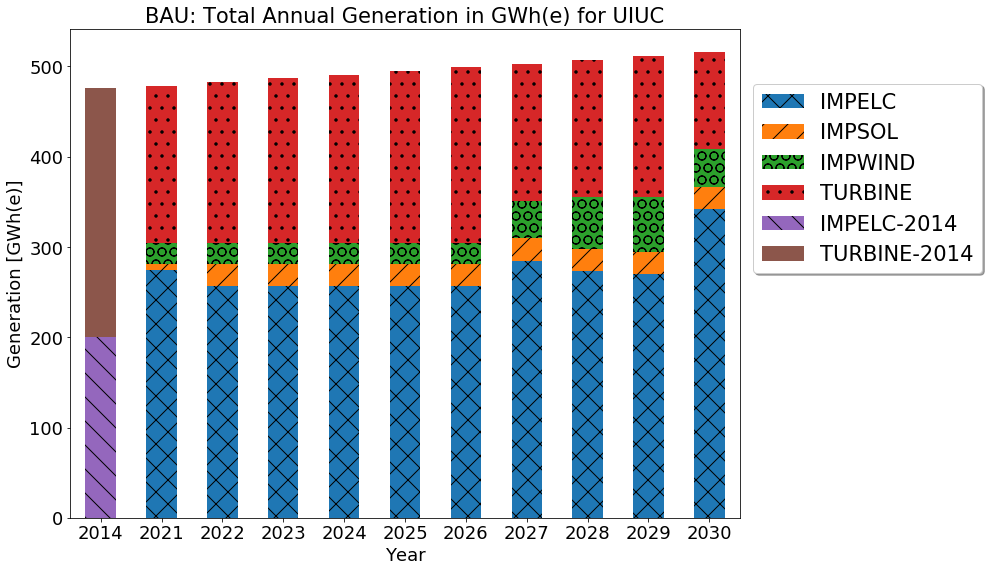
\includegraphics[width=\columnwidth]{bau_generation_w2014.png}
	\caption{Business as usual electricity generation.}
	\label{fig:bau_generation}
\end{figure}
\begin{figure}[H]
	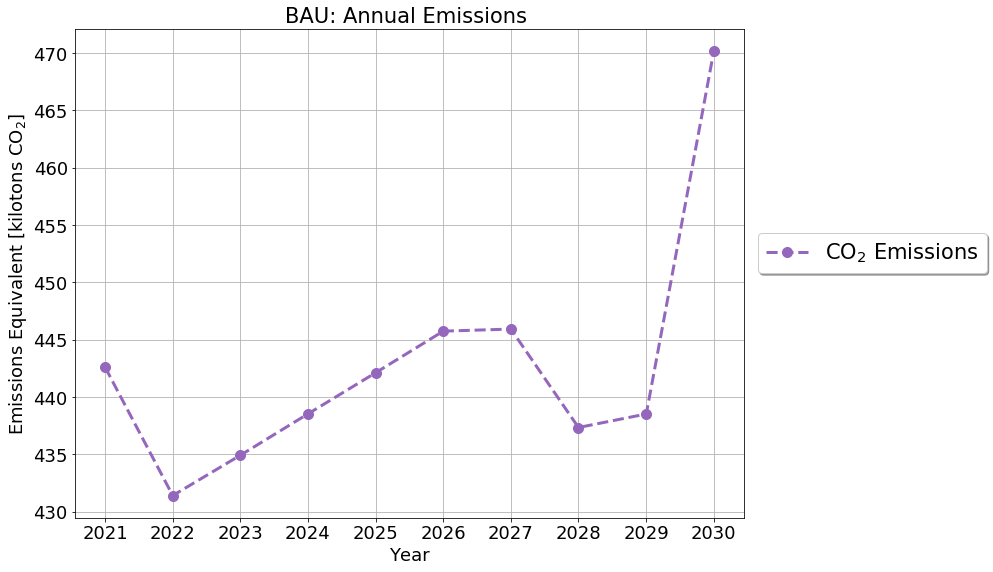
\includegraphics[width=\columnwidth]{bau_emissions.png}
	\caption{Business as usual carbon emissions.}
	\label{fig:bau_emissions}
\end{figure}
\subsection{Scenario 1}
\begin{figure}[H]
	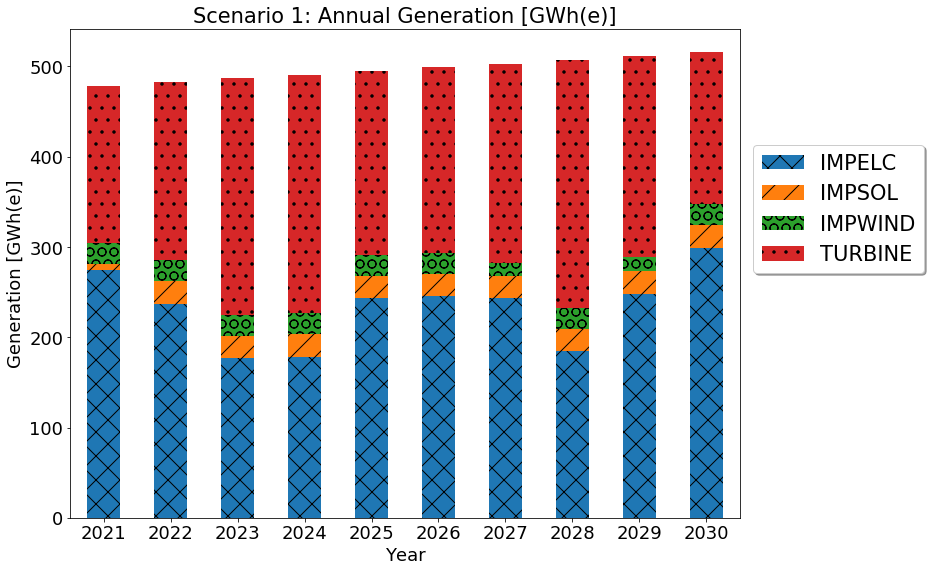
\includegraphics[width=\columnwidth]{scenario1_generation.png}
	\caption{Business as usual electricity generation.}
	\label{fig:}
\end{figure}
\begin{figure}[H]
	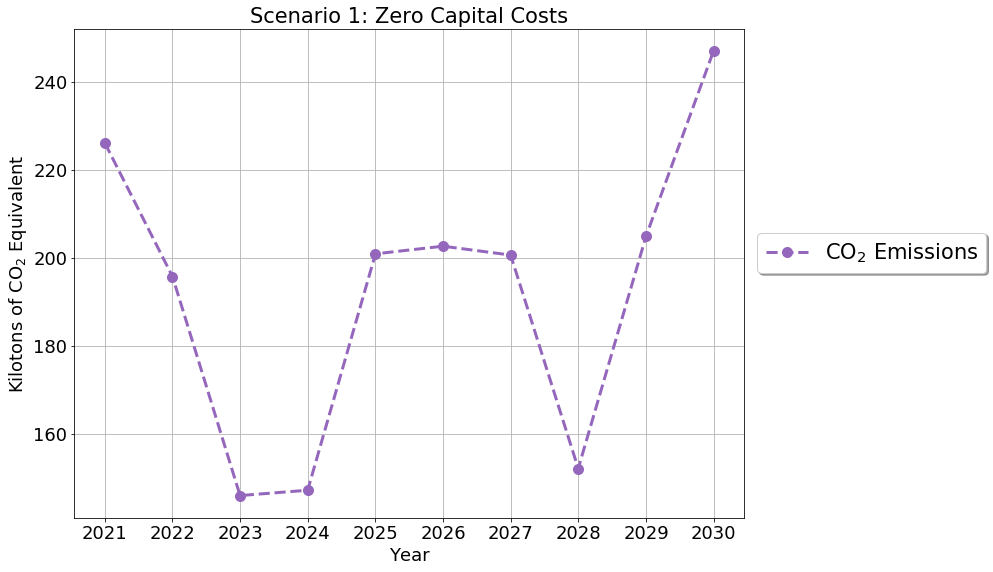
\includegraphics[width=\columnwidth]{scenario1_emissions.png}
	\caption{Business as usual electricity generation.}
	\label{fig:}
\end{figure}
\subsection{Scenario 2}
\begin{figure}[H]
	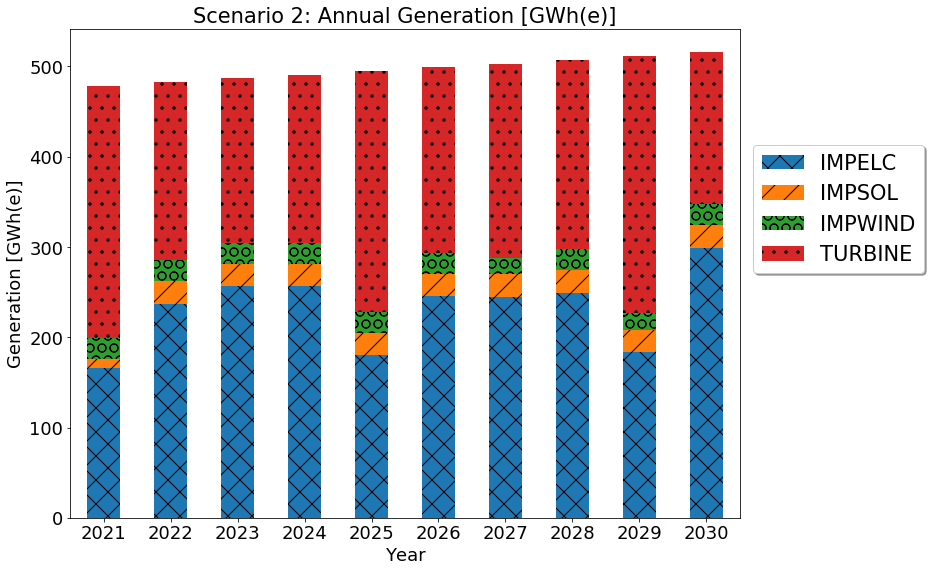
\includegraphics[width=\columnwidth]{scenario2_generation.png}
	\caption{Business as usual electricity generation.}
	\label{fig:}
\end{figure}
\begin{figure}[H]
	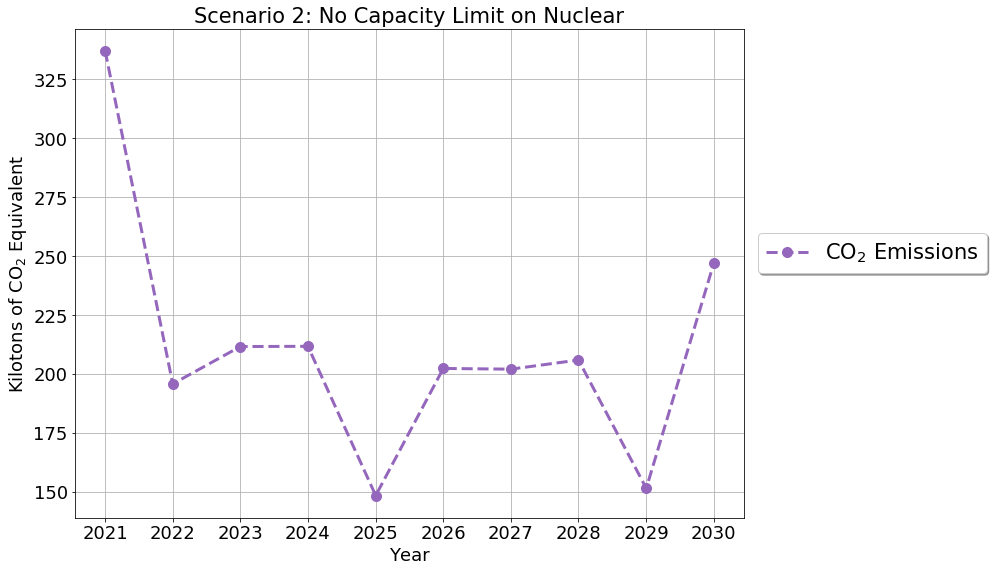
\includegraphics[width=\columnwidth]{scenario2_emissions.png}
	\caption{Business as usual electricity generation.}
	\label{fig:}
\end{figure}
\subsection{Scenario 3}
\begin{figure}[H]
	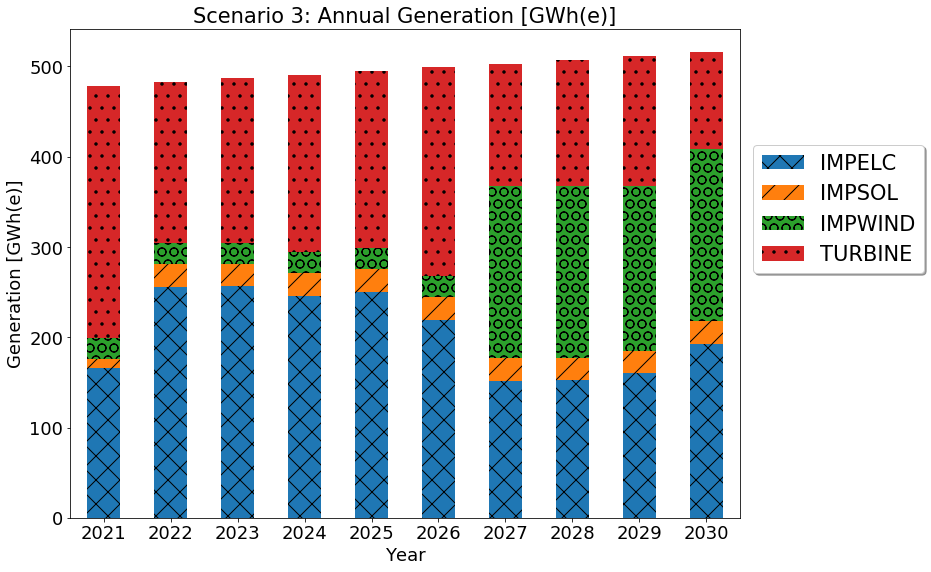
\includegraphics[width=\columnwidth]{scenario3_generation_elc.png}
	\caption{Business as usual electricity generation.}
	\label{fig:}
\end{figure}
\begin{figure}[H]
	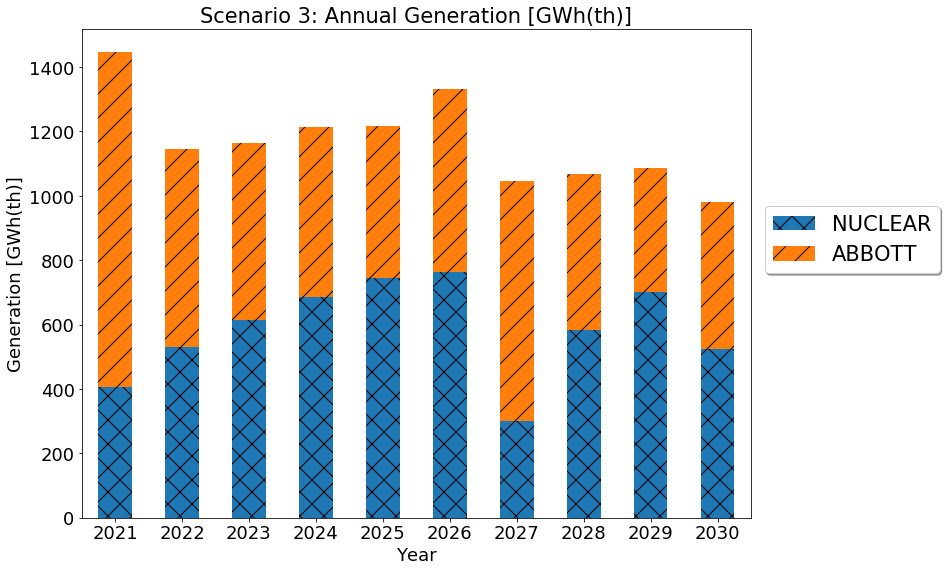
\includegraphics[width=\columnwidth]{scenario3_generation_stm.png}
	\caption{Business as usual electricity generation.}
	\label{fig:}
\end{figure}
\begin{figure}[H]
	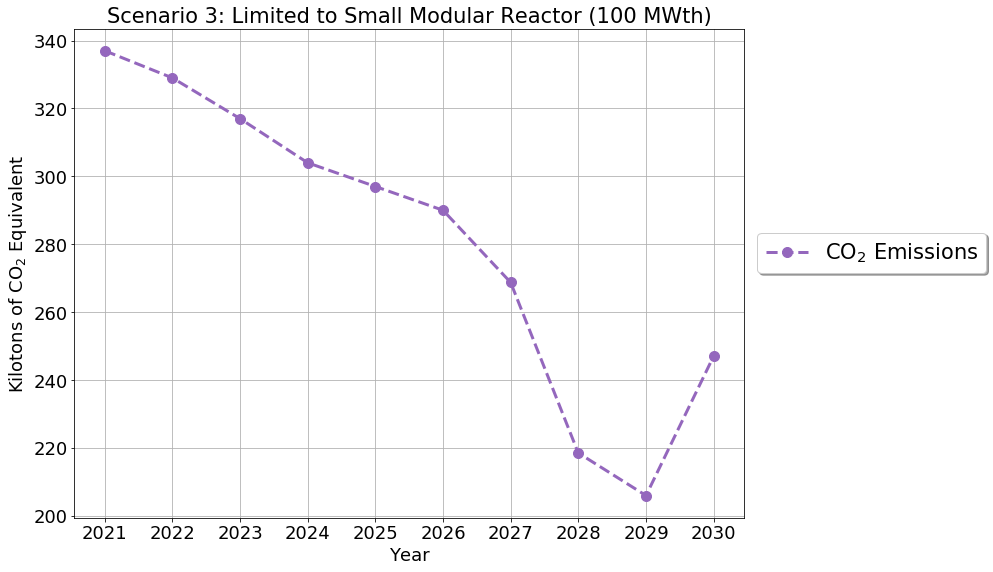
\includegraphics[width=\columnwidth]{scenario3_emissions.png}
	\caption{Business as usual electricity generation.}
	\label{fig:}
\end{figure}
\begin{figure}[H]
	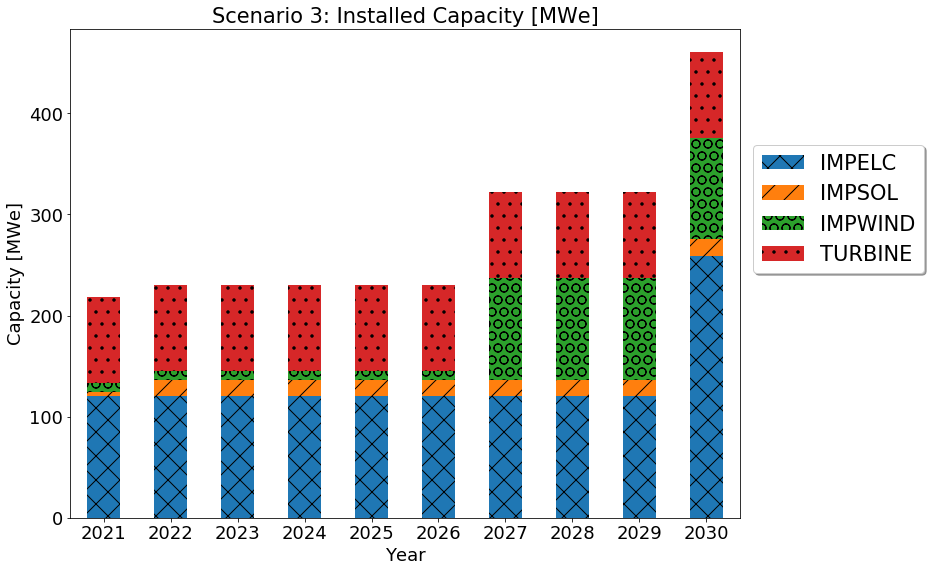
\includegraphics[width=\columnwidth]{scenario3_capacity_elc.png}
	\caption{Business as usual electricity generation.}
	\label{fig:}
\end{figure}
\begin{figure}[H]
	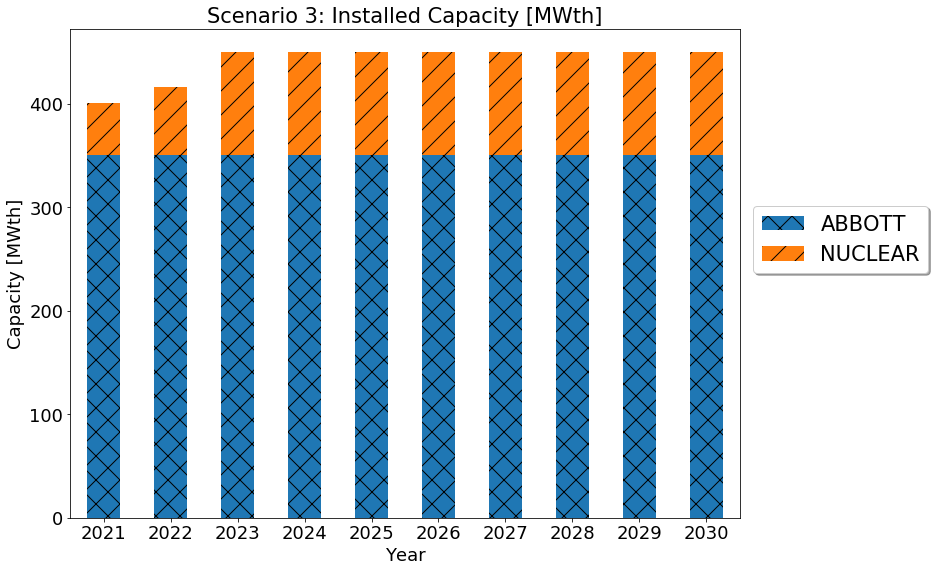
\includegraphics[width=\columnwidth]{scenario3_capacity_stm.png}
	\caption{Business as usual electricity generation.}
	\label{fig:}
\end{figure}
